% !TeX root = RJwrapper.tex
\title{Teaching Computers to See Patterns in Scatterplots with
Scagnostics}
\author{by Harriet Mason, Stuart Lee, Ursula Laa, and Dianne Cook}

\maketitle

\abstract{%
An abstract of less than 150 words.
}

\hypertarget{introduction}{%
\section{Introduction}\label{introduction}}

Visualising high dimensional data is often difficult and requires a
trade-off between the usefulness of the plots and maintaining the
structures of the original data. Scagnostics (scatterplot diagnostics)
are a set of visual features that can be used to identify interesting
and abnormal scatterplots, and thus give a sense of priority to the
variables we choose to visualise. This proposal will discuss the
creation of an R package that will provide a user-friendly method to
calculate these scagnostics. The package will be tested on datasets with
known interesting visual features to ensure the scagnostics are working
as expected, before finally being used to explore and describe a time
series dataset.

As the number of dimensions in a dataset increases, the process of
visualising its structure and variable dependencies becomes more
tedious. This is because the number of possible pairwise plots rises
exponentially with the number of dimensions. Datasets like Anscombe's
quartet \citep{anscombe} or the datasaurus dozen \citep{datasaurpkg}
have been constructed such that each pairwise plot has the same summary
statistics but strikingly different visual features. This design is to
illustrate the pitfalls of numerical summaries and the importance of
visualisation. This means that despite the issues that come with
increasing dimensionality, visualisation of the data cannot be ignored.
Scagnostics offer one possible solution to this issue.

The term scagnostics was introduced by John Tukey in 1982 \citep{tukey}.
Tukey discusses the value of a cognostic (a diagnostic that should be
interpreted by a computer rather than a human) to filter out
uninteresting visualisations. He denotes a cognostic that is specific to
scatter plots a scagnostic. Up to a moderate number of variables, a
scatter plot matrix (SPLOM) can be used to create pairwise
visualisations, however, this solution quickly becomes infeasible. Thus,
instead of trying to view every possible variable combination, the
workload is reduced by calculating a series of visual features, and only
presenting the outlier scatter plots on these feature combinations.

There is a large amount of research into visualising high dimensional
data, most of which focuses on some form of dimension reduction. This
can be done by creating a hierarchy of potential variables, performing a
transformation of the variables, or some combination of the two.
Unfortunately none of these methods are without pitfalls. Linear
transformations are subject to crowding, where low level projections
concentrate data in the centre of the distribution, making it difficult
to differentiate data points \citep{crowding}. Non-linear
transformations often have complex parameterisations, and can break the
underlying global structure of the data, creating misleading
visualisations. While there are solutions within these methods to fix
these issues such as a burning sage tour for crowding
\citep{burningsage} or liminal package for maintaining global structure
\citep{liminal} all these methods still involve some transformation of
the data. Scagnostics gives the benefit of allowing the user to view
relationships between the variables in their raw form. This means they
are not subject to the linear transformation issue of crowding, or the
non-linear transformation issue of misleading global structures. That
being said, only viewing pairwise plots can leave our variable
interpretations without context. Methods such as those shown in
\emph{ScagExplorer} \citep{scagexplorer} try to address this by
visualising the pairwise plots in relation to the scagnostic measures
distribution, but ultimately the lack of context remains one of the
limitations of using scagnostics alone as a dimension reduction
technique.

Scagnostics are not only useful in isolation, they can be applied in
conjunction with other techniques to find interesting feature
combinations of the transformed variables. The tourr projection pursuit
currently uses a selection of scagnostics to identify interesting low
level projections and move the visualisation towards them
\citep{tourrpp}. Since scagnostics are not dependent on the type of
data, they can also be used to compare and contrast scatter plots
regardless of the discipline. In this way, they are a useful metric for
something like the comparisons described in \emph{A self-organizing,
living library of time-series data}, which tries to organise time series
by their features instead of on their metadata \citep{sots}.

Several scagnostics have been previously defined in
\emph{Graph-Theoretic Scagnostics} \citep{scag}, which are typically
considered the basis of the visual features. They were all constructed
to range {[}0,1{]}, and later scagnostics have maintained this scale.
The formula for these measures were revised in \emph{Scagnostic
Distributions} and are still calculated according to this paper
\citep{scagdist}. In addition to the main nine, the benefit of using two
additional association scagnostics were discussed in Katrin Grimm's PhD
thesis \citep{Grimm}. These two association measures are also used in
the tourr projection pursuit \citep{tourrpp}.

There are two existing scagnostics packages, \emph{scagnostics}
\citep{scagdist} and the archived package \emph{binostics}
\citep{binostics}. Both are based on the original C++ code from
\emph{Scagnostic Distributions} \citep{something}, which is difficult to
read and difficult to debug. Thus there is a need for a new
implementation that enables better diagnosis of the scagnostics, and
better graphical tools for examining the results.

This paper describes the R package, \texttt{cassowaryr} that computes
the currently existing scagnostics, and adds several new measures. The
paper is organised as follows. The next section explains the
scagnostics. This is followed by a description of the implementation.
Several examples using collections of time series and XXX illustrate the
usage.

\hypertarget{scagnostics}{%
\section{Scagnostics}\label{scagnostics}}

\hypertarget{building-blocks-for-the-graph-based-metrics}{%
\subsection{Building blocks for the graph-based
metrics}\label{building-blocks-for-the-graph-based-metrics}}

In order to capture the visual structure of the data, graph theory is
used to calculate most of the scagnostics. The pairwise scatter plot is
re-constructed as a graph with the data points as vertices and the edges
are calculated using Delaunay triangulation. In the package this
calculation is done using the alphahull package \citep{alphahull} to
construct an object called a scree. This is the basis for all the other
objects that are used to calculate the scagnostics (except for
monotonic, dcor and splines which use the raw data). The graph (screen
object) is then used to construct the three key structures on which the
scagnostics are based; the convex hull, alpha hull and minimum-spanning
tree (MST).

\begin{itemize}
\item
  \textbf{Convex hull:} The outside vertices of the graph, connected to
  make a convex polygon that contains all points. It is constructed
  usnig the tripack package.
\item
  \textbf{Alpha hull:} A collection of boundaries that contain all the
  points in the graph. Unlike the convex hull, it does not need to be
  convex. It is calculated using the alphahull package
  \citep{alphahull}.
\item
  \textbf{MST:} the minimum spanning tree, i.e the smallest distance of
  branches that can be used to connect all the points. In the package it
  is calculated from the graph using the igraph package \citep{igraph}.
\end{itemize}

\begin{Schunk}
\begin{figure}
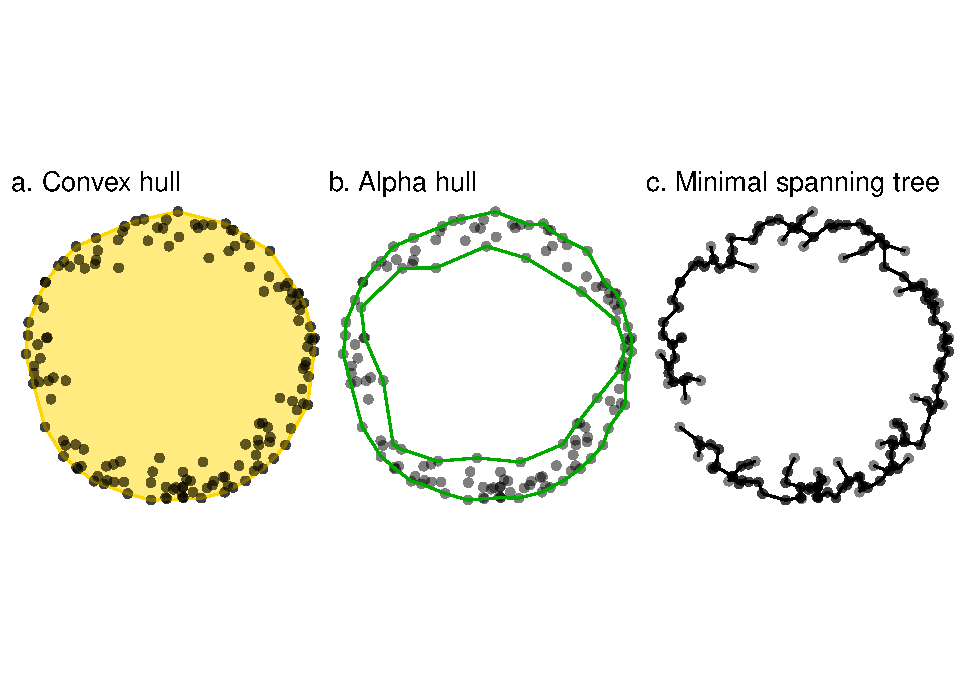
\includegraphics[width=1\linewidth]{mason-lee-laa-cook_files/figure-latex/building-blocks2-1} \caption[The building blocks for graph-based scagnostics]{The building blocks for graph-based scagnostics}(\#fig:building-blocks2)
\end{figure}
\end{Schunk}

\hypertarget{graph-based-scagnostics}{%
\subsection{Graph-based scagnostics}\label{graph-based-scagnostics}}

The nine scagnostics defined in \emph{Scagnostic Distributions} are
detailed below with an explanation, formula, and visualisation. We will
let \emph{A}= alpha Hull \emph{C}= convex hull, \emph{M} = minimum
spanning tree, and \emph{s}= the scagnostic measure. Since some of the
measures have some sample size dependence, we will let \emph{w} be a
constant that adjusts for that.

\begin{itemize}
\tightlist
\item
  \textbf{Convex:} Measure of how convex the shape of the data is.
  Computed as the ratio between the area of the alpha hull (A) and
  convex hull (C).
\end{itemize}

\[s_{convex}=w\frac{area(A)}{area(C)}\]


\includegraphics{figures/drawconvex.png}

\begin{itemize}
\tightlist
\item
  \textbf{Skinny:} A measure of how ``thin'' the shape of the data is.
  It is calculated as the ratio between the area and perimeter of the
  alpha hull (A) with some normalisation such that 0 correspond to a
  perfect circle and values close to 1 indicate a skinny polygon.
\end{itemize}

\[s_{skinny}= 1-\frac{\sqrt{4\pi area(A)}}{perimeter(A)}\]


\includegraphics{figures/drawskinny.png}

\begin{itemize}
\tightlist
\item
  \textbf{Outlying:} A measure of proportion and severity of outliers in
  dataset. Calculated by comparing the edge lengths of the outlying
  points in the MST with the length of the entire MST.
\end{itemize}

\[s_{outlying}=\frac{length(M_{outliers})}{length(M)}\]


\includegraphics{figures/drawoutlying.png}

\begin{itemize}
\tightlist
\item
  \textbf{Stringy:} This measure identifies a ``stringy'' shape with no
  branches, such as a thin line of data. It is calculated by comparing
  the number of vertices of degree two (\(V^{(2)}\)) with the total
  number of vertices (\(V\)), dropping those of degree one
  (\(V^{(1)}\)).
\end{itemize}

\[s_{stringy} = \frac{|V^{(2)}|}{|V|-|V^{(1)}|}\]

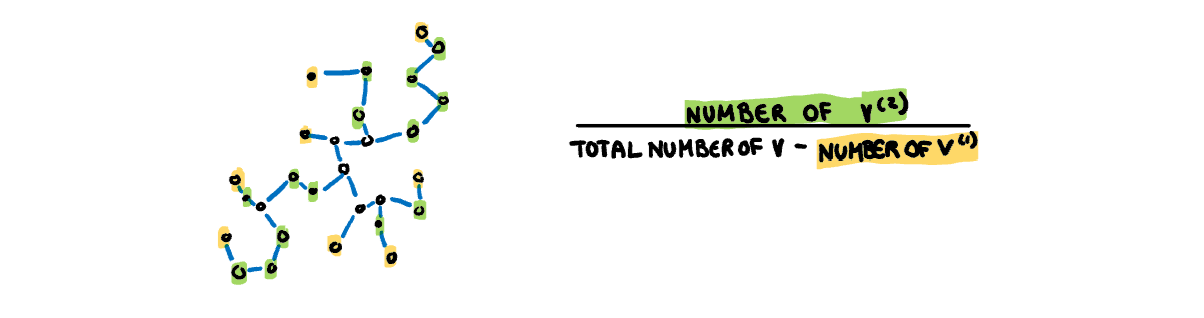
\includegraphics{figures/drawstringy.png}

\begin{itemize}
\tightlist
\item
  \textbf{Skewed:} A measure of skewness in the edge lengths of the MST
  (not in the distribution of the data). It is calculated as the ratio
  between the 40\% IQR and the 80\% IQR, adjusted for sample size
  dependence.
\end{itemize}

\[s_{skewed} = 1-w(1-\frac{q_{90}-{q_{50}}}{q_{90}-q_{10}})\]

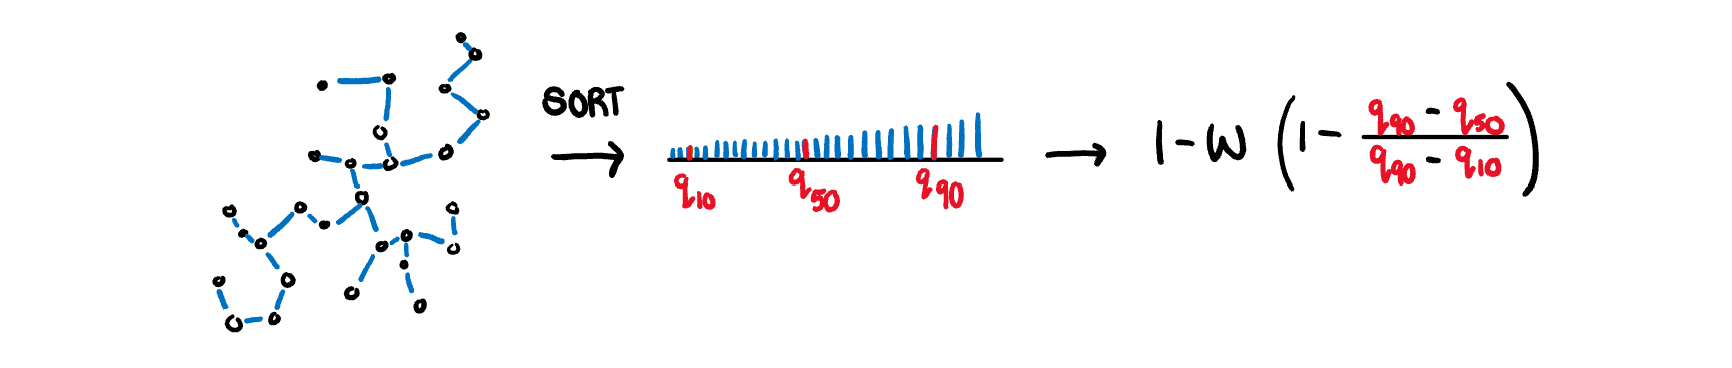
\includegraphics{figures/drawskewed.png}

\begin{itemize}
\tightlist
\item
  \textbf{Sparse:} Identifies if the data is sporadically located on the
  plane. Calculated as the 90th percentile of MST edge lengths.
\end{itemize}

\[s_{sparse}= wq_{90}\]

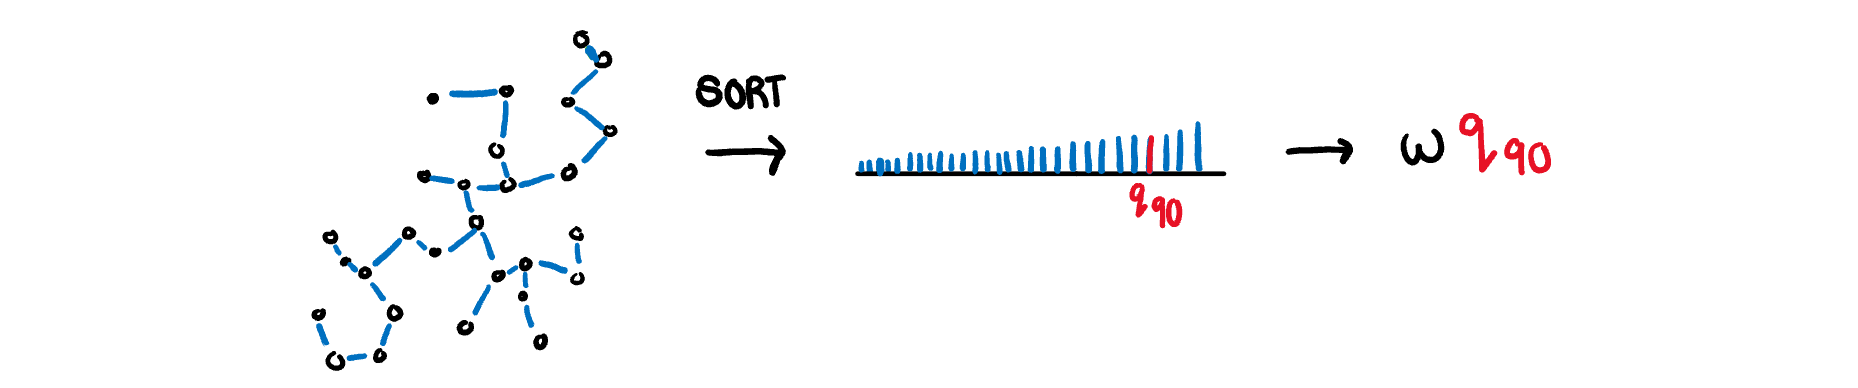
\includegraphics{figures/drawsparse.png}

\begin{itemize}
\tightlist
\item
  \textbf{Clumpy:} This measure is used to detect clustering and is
  calculated through an iterative process. First an edge J is selected
  and removed from the MST. From the two spanning trees that are created
  by this break, we select the largest edge from the smaller tree (K).
  The length of this edge (K) is compared to the removed edge (J) giving
  a clumpy measure for this edge. This process is repeated for every
  edge in the MST and the final clumpy measure is the maximum of this
  value over all edges.
\end{itemize}

\[\max_{j}[1-\frac{\max_{k}[length(e_k)]}{length(e_j)}]\]\\
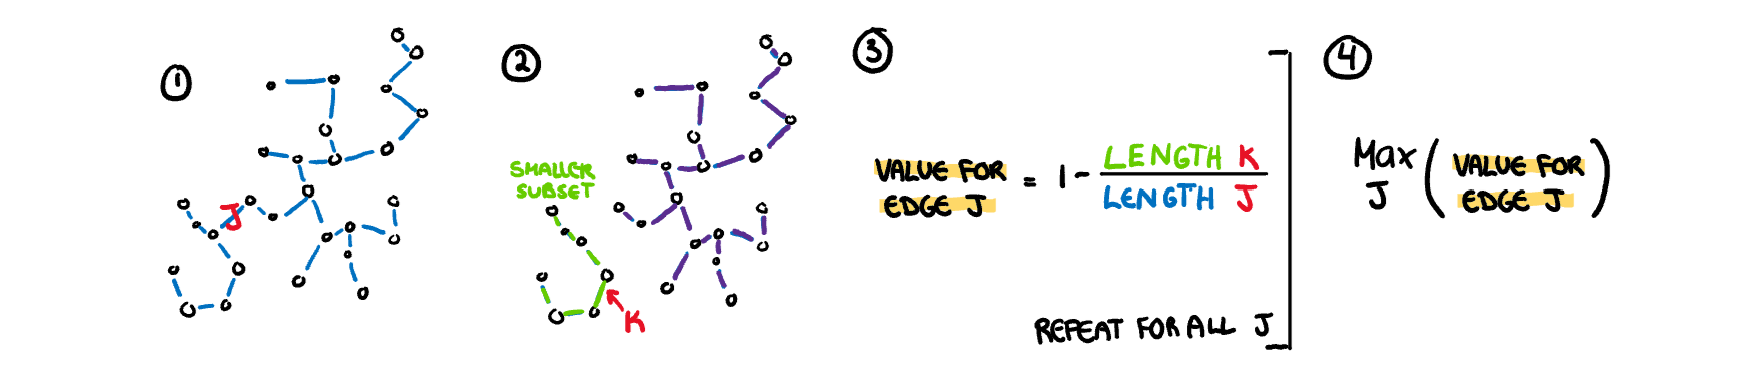
\includegraphics{figures/drawclumpy.png}

\begin{itemize}
\tightlist
\item
  \textbf{Striated:} This measure identifies features such as
  discreteness by finding parallel lines, or smooth algebraic functions.
  Calculated by counting the proportion of acute (0 to 40 degree) angles
  between the adjacent edges of vertices with only two edges.
\end{itemize}

\[\frac1{|V|}\sum_{v \in V^{2}}I(cos\theta_{e(v,a)e(v,b)}<-0.75)\]\\
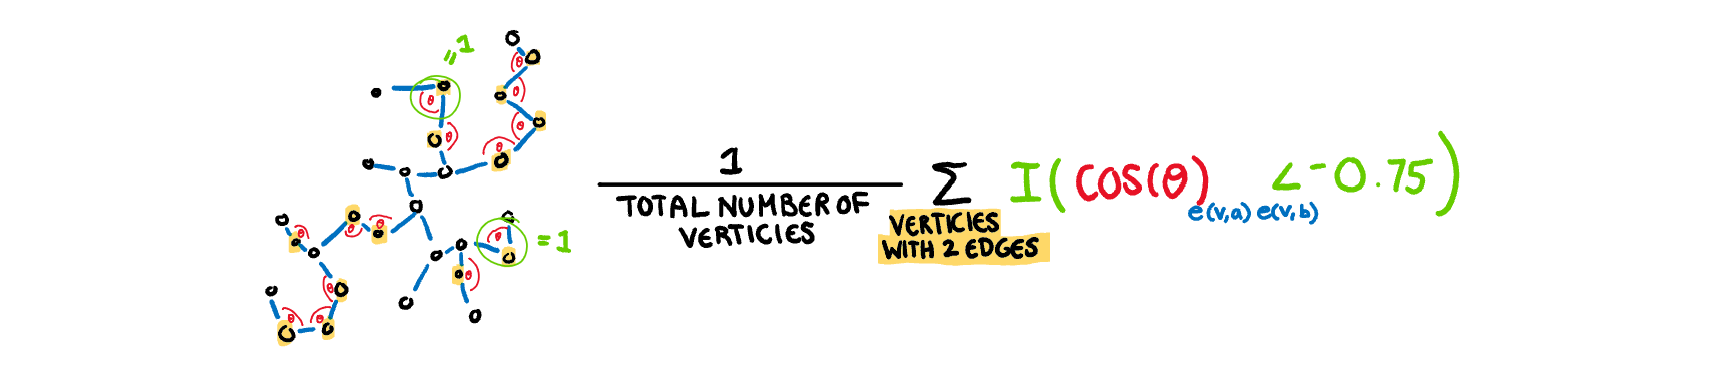
\includegraphics{figures/drawstriated.png}

\begin{itemize}
\tightlist
\item
  \textbf{Monotonic:} Checks if the data has an increasing or decreasing
  trend. Calculated as the Spearman correlation coefficient, i.e.~the
  Pearson correlation between the ranks of x and y.
\end{itemize}

\[s_{monotonic} = r^2_{spearman}\]
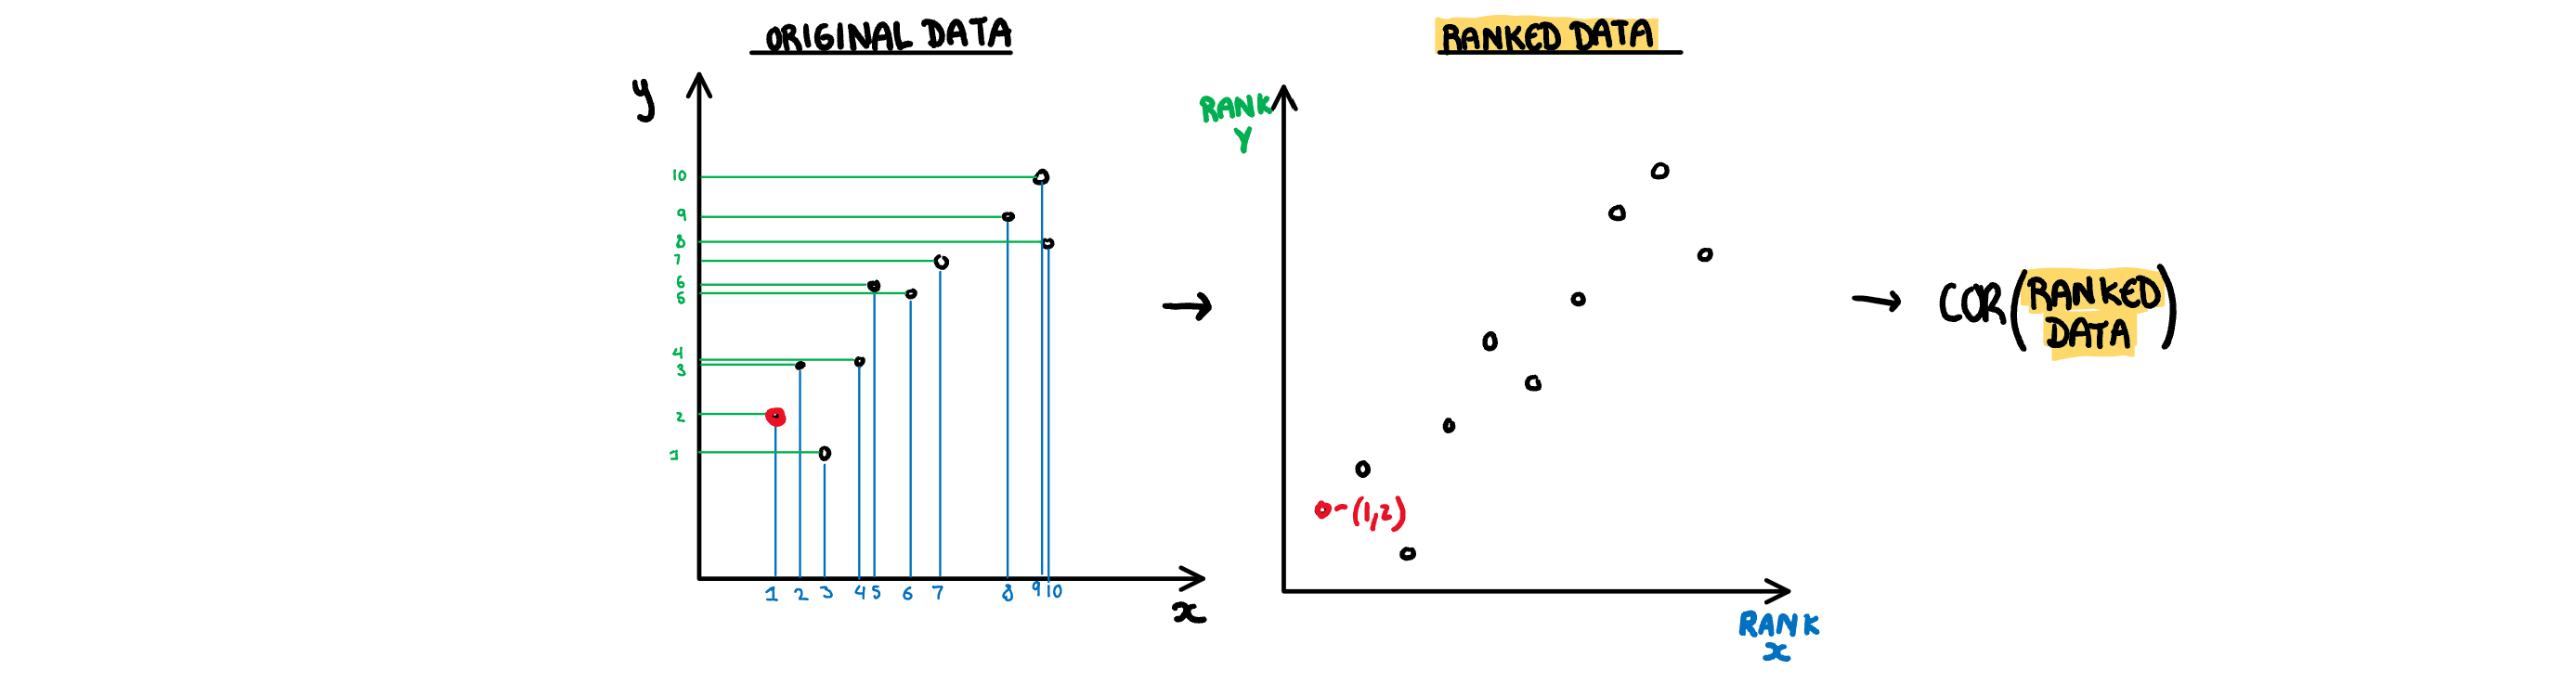
\includegraphics{figures/drawmonotonic.png}

\hypertarget{association-based-scagnostics}{%
\subsection{Association-based
scagnostics}\label{association-based-scagnostics}}

The two additional scagnostics discussed by Katrin Grimm are described
below.

\begin{itemize}
\tightlist
\item
  \textbf{Splines:} Measures the functional non-linear dependence by
  fitting a penalised splines model on X using Y, and on Y using X. The
  variance of the residuals are scaled down by the axis so they are
  comparable, and finally the maximum is taken. Therefore the value will
  be closer to 1 if either relationship can be decently explained by a
  splines model.
\end{itemize}

\[s_{splines}=\max_{i\in x,y}[1-\frac{Var(Residuals_{model~i=.})}{Var(i)}]\]

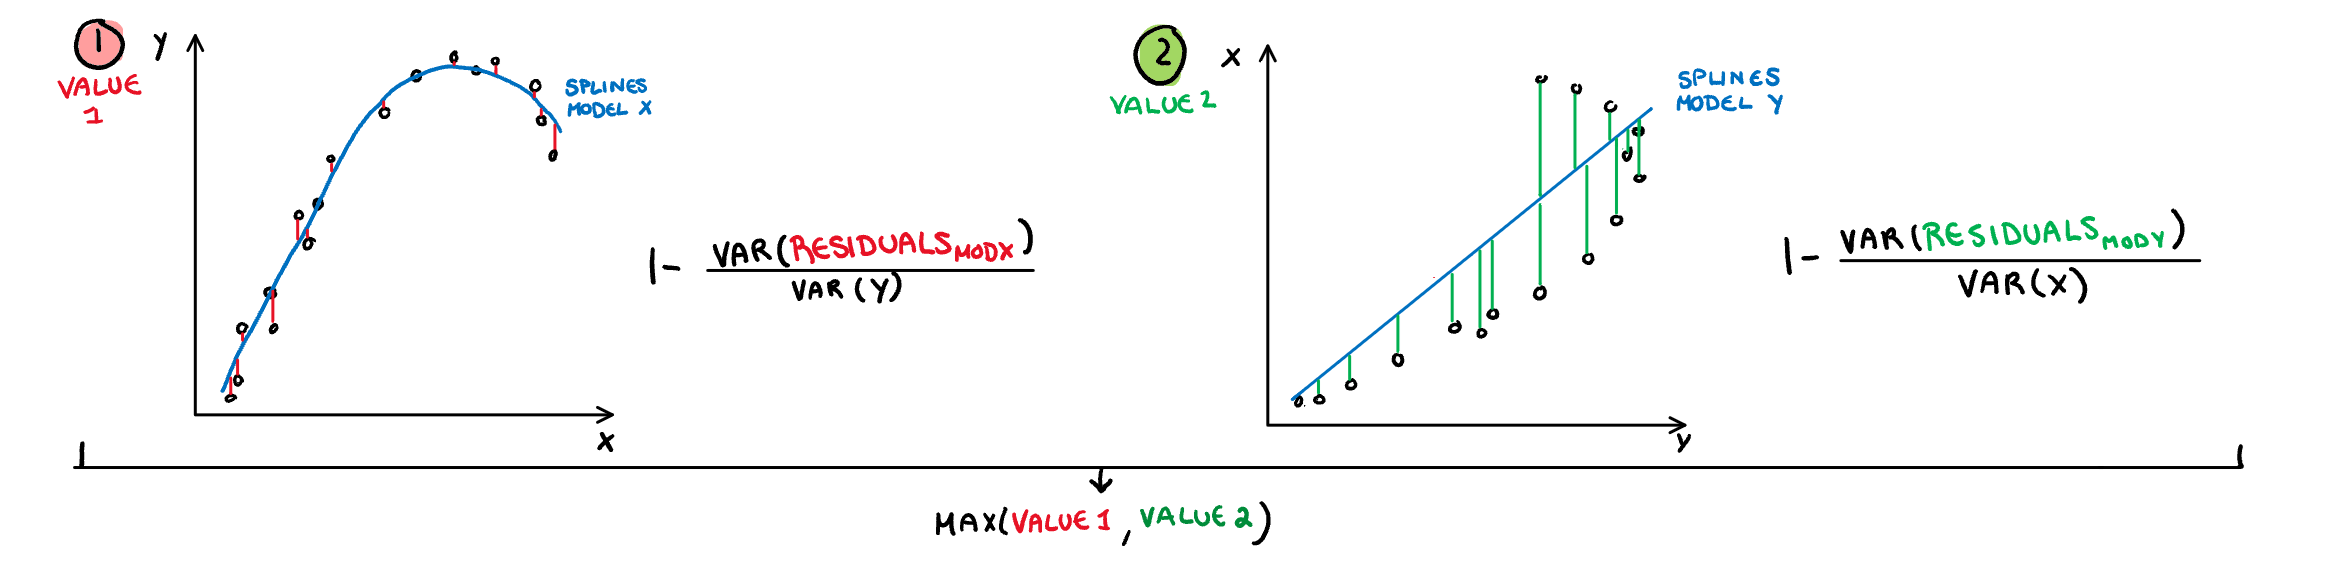
\includegraphics{figures/drawsplines.png}

\begin{itemize}
\tightlist
\item
  \textbf{Dcor:} A measure of non-linear dependence which is 0 if and
  only if the two variables are independent. Computed using an ANOVA
  like calculation on the pairwise distances between observations.
\end{itemize}

\[s_{dcor}= \sqrt{\frac{\mathcal{V}(X,Y)}{\mathcal{V}(X,X)\mathcal{V}(Y,Y)}}\]\\
where \[\mathcal{V}
(X,Y)=\frac{1}{n^2}\sum_{k=1}^n\sum_{l=1}^nA_{kl}B_{kl}\]\\
where \[A_{kl}=a_{kl}-\bar{a}_{k.}-\bar{a}_{.j}-\bar{a}_{..}\]
\[B_{kl}=b_{kl}-\bar{b}_{k.}-\bar{b}_{.j}-\bar{b}_{..}\]

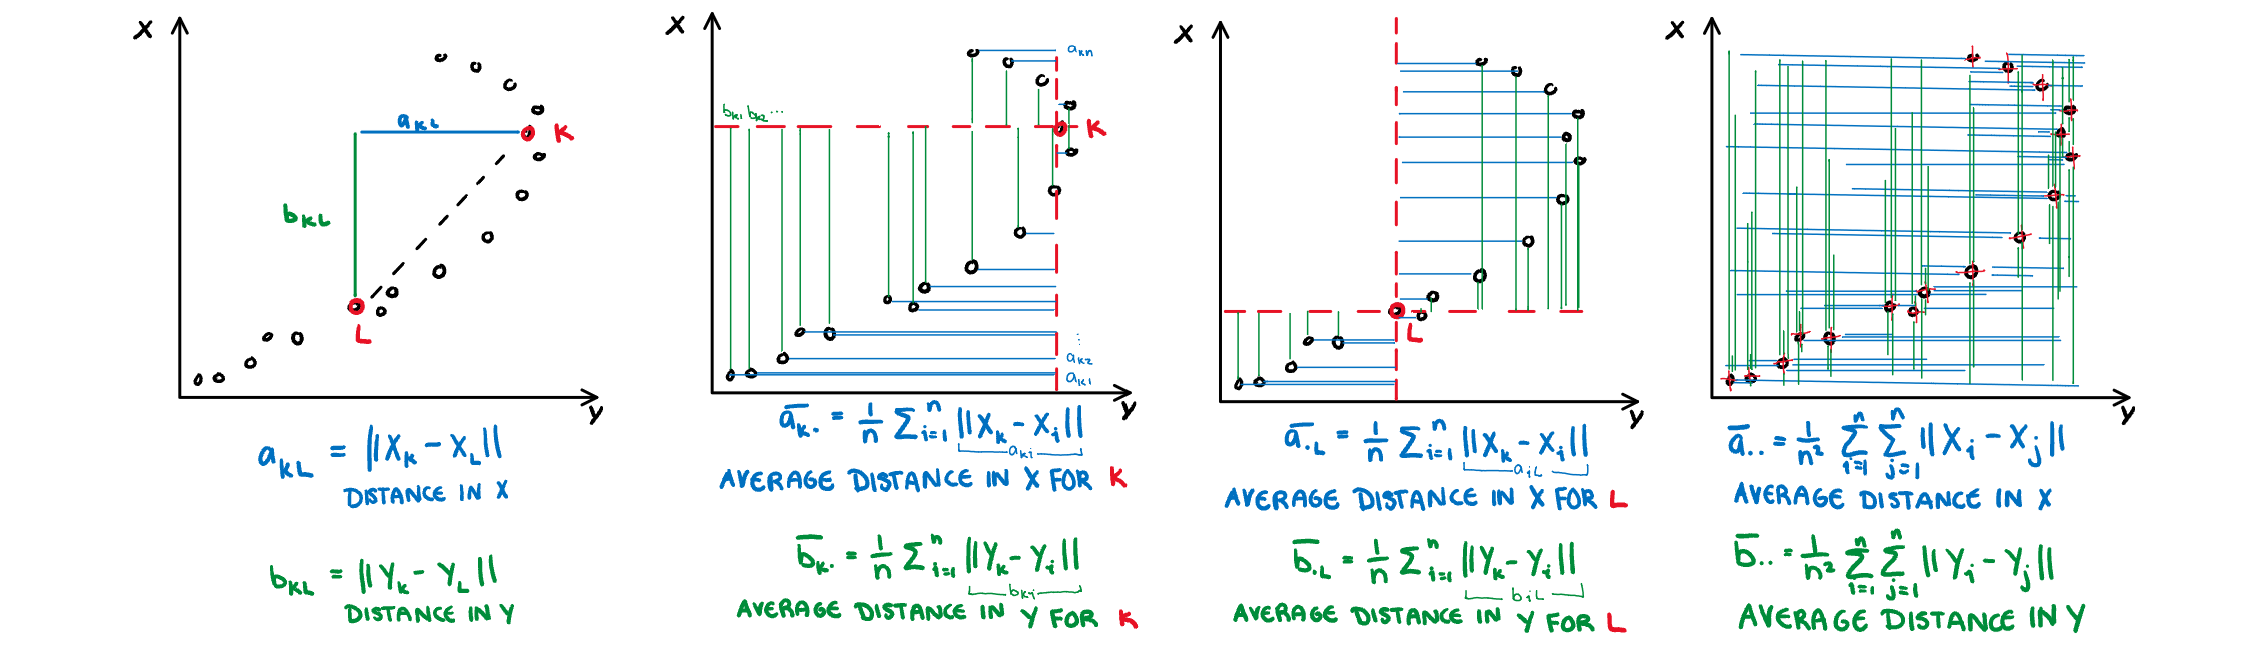
\includegraphics{figures/drawdcor.png}

\hypertarget{checking-the-scagnostics-calculations}{%
\subsection{Checking the scagnostics
calculations}\label{checking-the-scagnostics-calculations}}

Once we have written the scagnsotics by their definition and working
functions that correctly calculate them, we can assess how well they
identify the visual features of scatter plots. To assess how well the
scagnostics differentiate plots, we have creates a dataset called
``features'' (that is also in the Cassowaryr package) that contains a
series of interesting and unique scatter plots which we can run our
scagnsotics on.

\begin{Schunk}

\includegraphics{mason-lee-laa-cook_files/figure-latex/Features plot-1} \end{Schunk}

If we run these

While the scagnsotics can be shown to sort reasonably well within
themselves, is is entirely different to correctly sort the scatter plots
by what you would visually conclude.

\hypertarget{software-implementation}{%
\section{Software implementation}\label{software-implementation}}

\hypertarget{installation}{%
\subsection{Installation}\label{installation}}

\hypertarget{data-sets}{%
\subsection{Data sets}\label{data-sets}}

\hypertarget{functions}{%
\subsection{Functions}\label{functions}}

\hypertarget{scagnostics-functions}{%
\subsubsection{Scagnostics functions}\label{scagnostics-functions}}

\hypertarget{drawing-functions}{%
\subsubsection{Drawing functions}\label{drawing-functions}}

\hypertarget{summary-functions}{%
\subsubsection{Summary functions}\label{summary-functions}}

\hypertarget{tests}{%
\subsection{Tests}\label{tests}}

\hypertarget{examples}{%
\section{Examples}\label{examples}}

\hypertarget{collections-of-time-series}{%
\subsection{Collections of time
series}\label{collections-of-time-series}}

GOAL: Use scagnostics to find difference in shapes between groups. Here
we want to first use features to describe a time series, and then
secondly choosing pairs of features where there is the biggest
difference between groups according to a scagnostic.

A paragraph describing the compenginets data

Analysis notes:

\begin{itemize}
\tightlist
\item
  A big collection of time series. How do we understand the range of
  types of time series?
\item
  Calculate time series features. Using tsfeatures this will give 13
  values for each time series.
\item
  Use scagnostics to find pairs of tsfeatures that are interesting, eg
  high on splines but low on monotonic
\item
  Plot the pair of tsfeatures, what's unusual about the two?
\item
  Select unusual series from the tsfeatures, and plot
\end{itemize}

\hypertarget{compare-two-sets-of-time-series}{%
\subsubsection{Compare two sets of time
series}\label{compare-two-sets-of-time-series}}

This analysis compares the features of macroeconomic and microeconomic
series, using scagnostics. The goal of the comparison is to compare
shapes, not necessarily centres of groups as might be done in LDA or
other machine learning methods.

Here, just a small set of features is examined (because code fragile)
but what emerges as interesting is the difference between curvature and
trend strength. Microeconomic series tend to have high values on trend
strength, and a range of values on curvature. In comparison
macroeconomic series tend to have near constant average values on
curvature, and highly varied on trend strength.

Plotting a few series actually suggests that the microeconomic series
contain lots of micro structure, which might be what we should expect.
Interestingly the trend strength seems to pick up the jaggies!

\begin{Schunk}

\includegraphics{mason-lee-laa-cook_files/figure-latex/unnamed-chunk-3-1} \end{Schunk}

\begin{Schunk}

\includegraphics{mason-lee-laa-cook_files/figure-latex/unnamed-chunk-4-1} \end{Schunk}

\hypertarget{parkinsons}{%
\subsection{Parkinsons}\label{parkinsons}}

\hypertarget{black-hole-mergers}{%
\subsection{Black hole mergers}\label{black-hole-mergers}}

This is a simulated dataset that contains posterior samples for
describing an observed gravitational waves signal from a black hole
merger in terms of position in the sky (ra, dec, distance), time of the
event (time) and the black hole properties (masses m1 and m2; spin
related properties alpha, theta\_jn, chi\_tot, chi\_eff, chi\_p) and
additional nuisance parameters psi (polarisation angle) and phi\_jl
(orbital phase). There are thus 13 variables and it is still feasible to
look at a complete SPLOM, providing a good cross check of the
scagnostics.

The data contains 9998 posterior samples, without binning it is too long
to compute the scagnostics on such a large number of observations. For
our purpose a much smaller sample is sufficient, and we randomly sample
200 observations before computing the scagnostics.

Combinations that stand out: time-ra, dec-ra, dec-time (low convex, high
skinny) dec-ra and time-ra also have higher splines than dcor (both
high, non-linear functional relation), while m1-m2, dec-time and
chi\_p-chi\_tot have higher dcor than splines (still both high, m1-m2
and chi\_p-chi\_tot are linear relations with noise, dec-time is strong
association but not function) The final plot is showing clumpy vs
skewed, shows that clumpy isn't really doing what we expect since we
would expect much more structure in clumpy (in particular plots with
time break up into two well separated groups, plots with ra in three
separated groups, some other variables introduce less pronounced
separation between groups). Included time-alpha as one example, this has
clumpy of 0.9 and skewed of 0.7.

\hypertarget{afl-player-statistics}{%
\subsection{AFL player statistics}\label{afl-player-statistics}}

Some explanation of AFL, and about the AFLW competition. Particularly
explain any stats used in the plots: goals, kicks, posessions, \ldots{}

The Australian Football League Women's (AFLW) is the national
semi-profesisonal Australia Rules football league for female players.
Here we will analyse data sourced from the official AFL website with
information on the 2020 season, in which the league had 14 teams and
1932 players. There are 68 variables, 38 of which are numeric. The
others are categorical, like the players names or match ids, which would
not be used in scagnostic calculations. These numeric variables are
recorded per player per game: - \emph{timeOnGroundPercentage}:
percentage of the game the player was on the field.\\
- \emph{goals}: the 6 points a team gets when the kick the ball between
the two big posts.\\
- \emph{behinds}: the 1 point a team gets when they kick the ball
between the big post and small post.\\
- \emph{kicks}: number of kicks done by the player in this game.\\
- \emph{handballs}: number of handballs does by the player in the
game.\\
- \emph{disposals}: the number kicks and handballs a player has.\\
- \emph{marks}: total number of marks in the game (the ball travels more
than 15m and the player catches it without another player touching it or
it hitting the ground).\\
- \emph{bounces}: the number of times a player bounced the ball in a
game. A player must bounce the ball if they travel more than 15m and
they can only bounce the ball once.\\
- \emph{tackles}: Number of tackles performed by the player.\\
- \emph{contestedPossessions}: the number of disposals a player has
under pressure, i.e if a player is getting tackled and the get a
handball or kick out of the scuffle.\\
- \emph{uncontestedPossessions}: the number of disposals a player has
under no pressure where they have space and time to get rid of the
ball.\\
- \emph{totalPossessions}: The total number of time the player has the
ball. - \emph{inside50s}: the number of times the player has the ball
within the 50m arc around the oponents goals.\\
- \emph{marksInside50}: the number of marks a player gets within the 50m
arc around the oponents goals.\\
- \emph{contestedMarks}: the number of marks a player has under
pressure. - \emph{hitouts}: this is how many times a player or team taps
or punching the ball from a stoppage. - \emph{onePercenters}: all the
things a player can do without registering a disposal. Eg. Spoils
(punching the ball to stop someone from marking it), Shepparding
(blocking for a teammate), smothering.\\
disposalEfficiency: a measure of how well a player disposes of the ball.
E.g. if a player kicks or handballs to the opposition a lot, they will
have a low disposal efficiency percentage.\\
- \emph{clangers}: this is how many times a player or team dispose of
the ball and it results in a turnover to the other team.\\
- \emph{freesFor}: this player was awarded a free kick.\\
- \emph{freesAgainst}: this player caused a free kick to be awarded to
the other team.\\
- \emph{dreamTeamPoints}: this is fantasy football scoring points.\\
- \emph{rebound50s}: how many times the player exits the ball out of
their defence 50m arc.\\
- \emph{goalAssists}: number of times the player gave the pass
immediately before the player that scored a goal. - \emph{goalAccuracy}:
percentage ratio of the number of goals kicked to the number of goal
attempts.\\
- \emph{turnovers}: this players disposal caused a turnover (the ball
touches the ground and the other team get it).\\
- \emph{intercepts}: number of times this player intercepts the disposal
of the other team. - \emph{tacklesInside50}: number of tackles performed
by this player within their defence 50m arc.\\
- \emph{shotsAtGoal}: number of total shots at goal for this player (sum
of goals, behinds and misses) - \emph{scoreInvolvements}: number of
times the player was involved in a passage of play leading up to a goal.
- \emph{metresGained}: how far a player has been able to advance the
ball without turning it over.\\
- \emph{clearances.centreClearances}: this is the clearance from the
centre bounce after a goal or at the start of a quarter -
\emph{clearances.stoppageClearances}: all the clearance from stoppages
around the ground - \emph{clearances.totalClearances}: how many time a
player or team clears the ball from a stoppage or from the centre

With 38 variables, there are 703 possible scatterplots to make. The
scagnostics can suggest which are the interesting ones to examine.

\begin{Schunk}


|Var1                       |Var2                          | splines|
|:--------------------------|:-----------------------------|-------:|
|totalPossessions           |disposals                     |    0.94|
|clearances.totalClearances |clearances.stoppageClearances |    0.88|
|goalAccuracy               |goals                         |    0.83|
|metresGained               |kicks                         |    0.77|
|dreamTeamPoints            |disposals                     |    0.74|
|disposals                  |kicks                         |    0.72|
|dreamTeamPoints            |totalPossessions              |    0.72|
|totalPossessions           |uncontestedPossessions        |    0.68|
|dreamTeamPoints            |kicks                         |    0.67|
|uncontestedPossessions     |disposals                     |    0.66|

\end{Schunk}

\begin{Schunk}
\begin{figure}
\includegraphics[width=1\linewidth]{mason-lee-laa-cook_files/figure-latex/aflwstatic-1} \caption[Scatterplots with high values on the splines scagnostic]{Scatterplots with high values on the splines scagnostic.}(\#fig:aflwstatic)
\end{figure}
\end{Schunk}

Figure @ref\{fig:aflwstatic\} shows three scatterplots that score highly
on the splines scagnostic. Each of these shows a relatively strong
monotonic relationship between the two variables. In the interactive
version of the plot, mouse over reveals some high-performing players,
e.g.~Anne Hatchard has a lot of possessions, disposals and kicks, and
Kaitlyn Ashmore kicked 4 goals in a match with 100\% accuracy.

NOTE: Each player is represented multiple times here, I think. The stats
are per game. Maybe it is better to aggregate for each player and re-do
the statistics?

The scagnsotics need to be used and interpreted with the type of dataset
you are working with in mind. For example, since these are sports stats,
almost all of the variables are discrete. This means in the case of the
striated varibale, we would be interested in the scatter plots that are
very low on striated rather than high. Lets see which striated measure
can find some interesting scatter plots.

Why the lowest values on striated? This is a discrete data set, if all
the points are not at right angles or in a stright line, to each other,
they are not just randonly spread on the. Since the old striated measure
is specifically trying to find a continuous variable against a discrete
variable, its highest values are also identified by the
striated\_adjusted. The lowest values on striated simply identify a plot
where all the variables are at right angles, once again a measure of
disceteness but one that is not identified by striated.
Striated\_adjusted encapsulates both versions of discreteness in the
values that get exactly a 1, this means the scatter plot that gets the
lowest value should be the two variables that are continuous. Following
that striated\_adjusted gives some interesting scatter plots in both
goal and dispsoal accuracy vs number. \textbf{comment on the scatter
plots}.

\hypertarget{world-development-indicators}{%
\subsection{World Development
Indicators}\label{world-development-indicators}}

The World Bank delivers a lot of development indicators, for many
countries and multiple years. This might be a good example to identify
pairs of indicators with interesting relationships.

Download data from:

\url{https://databank.worldbank.org/source/world-development-indicators/preview/on\#}

\begin{Schunk}
\begin{Soutput}
#>  Country Code        SP.ADO.TFRT     NV.AGR.TOTL.ZS   
#>  Length:31          Min.   : 1.320   Min.   : 0.5689  
#>  Class :character   1st Qu.: 5.783   1st Qu.: 1.6509  
#>  Mode  :character   Median :11.326   Median : 2.7612  
#>                     Mean   :22.601   Mean   : 5.0012  
#>                     3rd Qu.:33.681   3rd Qu.: 5.8037  
#>                     Max.   :82.313   Max.   :22.8556  
#>  EN.ATM.CO2E.PC    NE.EXP.GNFS.ZS    SP.DYN.TFRT.IN 
#>  Min.   : 0.5128   Min.   :  8.972   Min.   :0.977  
#>  1st Qu.: 3.2201   1st Qu.: 19.527   1st Qu.:1.565  
#>  Median : 5.5203   Median : 31.205   Median :1.730  
#>  Mean   : 6.3624   Mean   : 37.190   Mean   :1.805  
#>  3rd Qu.: 8.3006   3rd Qu.: 40.876   3rd Qu.:2.042  
#>  Max.   :15.4755   Max.   :122.298   Max.   :3.510  
#>  BX.KLT.DINV.CD.WD    AG.LND.FRST.K2    NY.GDP.MKTP.CD     
#>  Min.   :-3.615e+11   Min.   :    500   Min.   :2.622e+10  
#>  1st Qu.: 2.097e+09   1st Qu.:  34908   1st Qu.:3.601e+11  
#>  Median : 1.282e+10   Median : 144913   Median :9.136e+11  
#>  Mean   : 2.485e+10   Mean   : 800131   Mean   :2.291e+12  
#>  3rd Qu.: 5.845e+10   3rd Qu.: 627440   3rd Qu.:2.004e+12  
#>  Max.   : 2.615e+11   Max.   :8153116   Max.   :2.061e+13  
#>  NY.GDP.MKTP.KD.ZG NY.GNP.PCAP.CD  NY.GNP.PCAP.PP.CD
#>  Min.   :-2.565    Min.   : 1480   Min.   : 4750    
#>  1st Qu.: 1.548    1st Qu.: 9390   1st Qu.:17615    
#>  Median : 2.580    Median :32730   Median :42660    
#>  Mean   : 3.083    Mean   :31777   Mean   :37232    
#>  3rd Qu.: 3.960    3rd Qu.:48630   3rd Qu.:52645    
#>  Max.   : 8.516    Max.   :85030   Max.   :72330    
#>  NY.GNP.ATLS.CD      NY.GNP.MKTP.PP.CD   NE.GDI.TOTL.ZS 
#>  Min.   :2.390e+10   Min.   :1.952e+10   Min.   :14.95  
#>  1st Qu.:3.127e+11   1st Qu.:6.471e+11   1st Qu.:21.00  
#>  Median :8.831e+11   Median :1.659e+12   Median :24.08  
#>  Mean   :2.262e+12   Mean   :3.229e+12   Mean   :24.32  
#>  3rd Qu.:1.981e+12   3rd Qu.:3.076e+12   3rd Qu.:27.30  
#>  Max.   :2.076e+13   Max.   :2.162e+13   Max.   :43.79  
#>   SH.IMM.MEAS  
#>  Min.   :73.0  
#>  1st Qu.:92.5  
#>  Median :95.0  
#>  Mean   :94.1  
#>  3rd Qu.:97.0  
#>  Max.   :99.0
\end{Soutput}

\includegraphics{mason-lee-laa-cook_files/figure-latex/unnamed-chunk-13-1} 
\includegraphics{mason-lee-laa-cook_files/figure-latex/unnamed-chunk-13-2} \end{Schunk}

\hypertarget{summary}{%
\subsection{Summary}\label{summary}}

\begin{verbatim}
\end{verbatim}

\bibliography{mason-lee-laa-cook.bib}

\address{%
Harriet Mason\\
Monash University\\%
Department of Econometrics and Business Statistics\\ Melbourne,
Australia\\
%
\url{https://www.britannica.com/animal/quokka}\\%
\textit{ORCiD: \href{https://orcid.org/0000-1721-1511-1101}{0000-1721-1511-1101}}\\%
\href{mailto:hmas0003@student.monash.edu}{\nolinkurl{hmas0003@student.monash.edu}}%
}

\address{%
Stuart Lee\\
Genentech\\%
\\
%
\url{https://stuartlee.org}\\%
\textit{ORCiD: \href{https://orcid.org/0000-0003-1179-8436}{0000-0003-1179-8436}}\\%
\href{mailto:stuart.andrew.lee@gmail.com}{\nolinkurl{stuart.andrew.lee@gmail.com}}%
}

\address{%
Ursula Laa\\
University of Natural Resources and Life Sciences\\%
Institute of Statistics\\ Vienna, Austria\\
%
\url{https://uschilaa.github.io}\\%
\textit{ORCiD: \href{https://orcid.org/0000-0002-0249-6439}{0000-0002-0249-6439}}\\%
\href{mailto:ursula.laa@boku.ac.at}{\nolinkurl{ursula.laa@boku.ac.at}}%
}

\address{%
Dianne Cook\\
Monash University\\%
Department of Econometrics and Business Statistics\\ Melbourne,
Australia\\
%
\url{https://dicook.org}\\%
\textit{ORCiD: \href{https://orcid.org/000-0002-3813-7155}{000-0002-3813-7155}}\\%
\href{mailto:dicook@monash.edu}{\nolinkurl{dicook@monash.edu}}%
}
